\documentclass{beamer}

\mode<presentation>
{
  \usetheme{CambridgeUS}
  \setbeamercovered{transparent}
  \setbeamertemplate{itemize items}[circle]
  \setbeamercolor{itemize item}{fg=red}%{\color{red}$\blacksquare$}
  \setbeamercolor{itemize subitem}{fg=gray}%{\color{gray}$\blacktriangleright$}
}

\usepackage[english]{babel}
\usepackage[latin1]{inputenc}
\usepackage{times}
\usepackage[T1]{fontenc}
\usepackage[font=small,labelfont=bf]{caption}
% Or whatever. Note that the encoding and the font should match. If T1
% does not look nice, try deleting the line with the fontenc.
\usepackage{amsmath}
\usepackage{hyperref}

\newcommand{\linespace}{\vskip 0.25cm}

%\definecolor{MyForestGreen}{rgb}{0,0.7,0} 
%\newcommand{\tableemph}[1]{{#1}}
%\newcommand{\tablewin}[1]{\tableemph{#1}}
%\newcommand{\tablemid}[1]{\tableemph{#1}}
%\newcommand{\tablelose}[1]{\tableemph{#1}}

%\definecolor{MyLightGray}{rgb}{0.6,0.6,0.6}
%\newcommand{\tabletie}[1]{\color{MyLightGray} {#1}}

% The text in square brackets is the short version of your title and will be used in the
% header/footer depending on your theme.
\title[Foveated Rendering]{Foveated rendering \\ in virtual reality}

% Sub-titles are optional - uncomment and edit the next line if you want one.
% \subtitle{Why does sub-tree crossover work?} 

% The text in square brackets is the short version of your name(s) and will be used in the
% header/footer depending on your theme.
\author[Miller]{Sam Miller}

% The text in square brackets is the short version of your institution and will be used in the
% header/footer depending on your theme.
\institute[U of Minn, Morris]
{
  Division of Science and Mathematics \\
  University of Minnesota, Morris \\
  Morris, Minnesota, USA
}

% The text in square brackets is the short version of the date if you need that.
\date[October '17] % (optional)
{October 2017}

% Delete this, if you do not want the table of contents to pop up at
% the beginning of each subsection:
%\AtBeginSection[]
%{
%  \begin{frame}<beamer>
%    \frametitle{Outline}
%    \tableofcontents[currentsection, hideothersubsections]
%  \end{frame}
%}

\begin{document}

\begin{frame}
  \titlepage
\end{frame}

% For a 20-25 minute senior seminar talk you probably want something like:
% - Two or three major sections (other than the summary).
% - At *most* three subsections per section.
% - Talk about 30s to 2min per frame. So there should probably be between
%   15 and 30 frames, all told.


\section[Introduction]{}

\begin{frame}

  \begin{center}
    \includegraphics[width=.90\textwidth]{Illustrations/normalPC.png}
  \end{center}
  
\end{frame}

\begin{frame}

  \begin{center}
    \includegraphics[width=.90\textwidth]{Illustrations/macSmallLight.png}
  \end{center}
  
\end{frame}

\begin{frame}

  \begin{center}
    \includegraphics[width=.90\textwidth]{Illustrations/macBigLight.png}
  \end{center}
  
\end{frame}

\begin{frame}

  \begin{center}
    \includegraphics[width=.90\textwidth]{Illustrations/1junglePC.png}
  \end{center}
  
\end{frame}

\begin{frame}
  \begin{center}
    \includegraphics[width=.90\textwidth]{Illustrations/2junglePC.png}
  \end{center}
  
\end{frame}

\begin{frame}

  %\end{column}
  \begin{center}
    \includegraphics[width=.90\textwidth]{Illustrations/junglePCPixel2.png}
  \end{center}
  
\end{frame}

\begin{frame}

  \begin{center}
    \includegraphics[width=.9\textwidth]{Illustrations/junglePCPixelSmoothed.png}
  \end{center}
  
\end{frame}


\begin{frame}

  \begin{center}
    \includegraphics[width=.90\textwidth]{Illustrations/1junglePC.png}
  \end{center}
  
\end{frame}

\begingroup

\setbeamercolor{background canvas}{bg=black}

\begin{frame}

  \begin{center}
    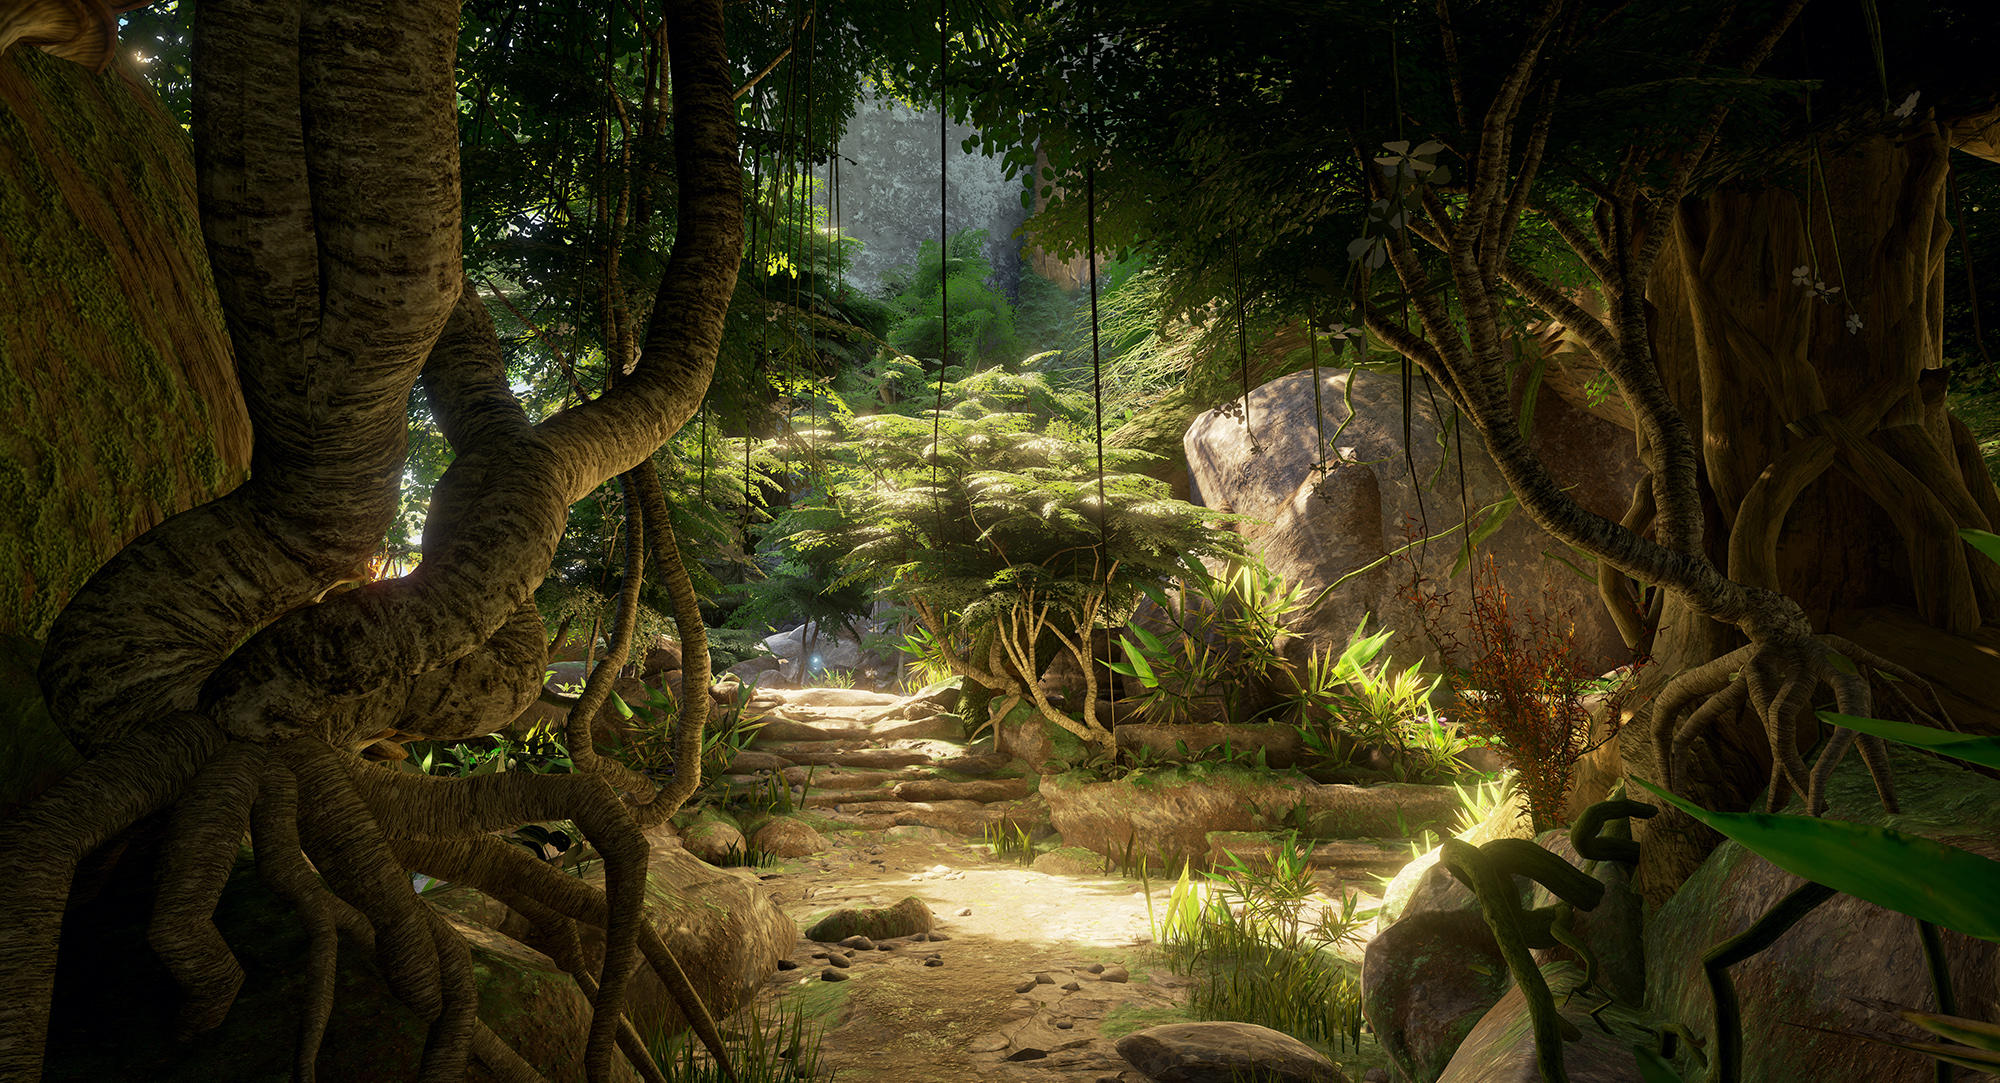
\includegraphics[width=4.7in]{Illustrations/jungle.jpg}
    \\
    %\tiny{Sam Fraser-Smith \\ \url{http://tr.im/pq7l} }
  \end{center}
  
\end{frame}

\endgroup

\section*{Overview}

\subsection*{Outline}

\begin{frame}
  \frametitle{Outline}
  	%\tableofcontents[hideallsubsections]
  	
	\begin{itemize}
    \item Background
	\begin{itemize}
    \item Human Vision
    \item Virtual Reality Headsets
    \item Gaze Tracking
    \linespace
	\end{itemize}
	\item Foveated Renderer Design
	\begin{itemize}
	\item Rendering Components
    \item Desktop Implementation
    \item VR Implementation
    \linespace
	\end{itemize}
	\item Results
	\linespace
	\item Conclusion
	\end{itemize}
	

\end{frame}

\section[Background]{Concepts}

\subsection{Human Vision}

\begin{frame}
  \frametitle{Visual Regions}
	\begin{itemize}
		\item Fovea
		\begin{itemize}
			\item center of vision
			\item high spatial density of photoreceptors
			\item Approximately 5 degrees in diameter 
		\end{itemize}
	\linespace
		\item Periphery
			\begin{itemize}
				\item distal region surrounding the fovea
				\item progressively lower spatial density of photoreceptors
				\item undersampled by optic nerve
			\end{itemize}
	\end{itemize}
\end{frame}

\begin{frame}
  \frametitle{Visual Acuity}
	\begin{itemize}
		\item Cortical Magnification Factor (CMF)
	\linespace
		\item Acuity Falloff
			\begin{itemize}
				\item corresponds to retinal eccentricity
				\item basis for foveal layer division
			\end{itemize}
	\end{itemize}
\end{frame}

\begin{frame}
  \frametitle{Saccadic Eye Movements}
	\begin{itemize}
		\item Disjunct leaping motion of the eyes to look at a new focal point
		\item Significant hurdle for Gaze Tracking and subsequently Foveated Rendering
	\end{itemize}
	
	  \begin{center}
    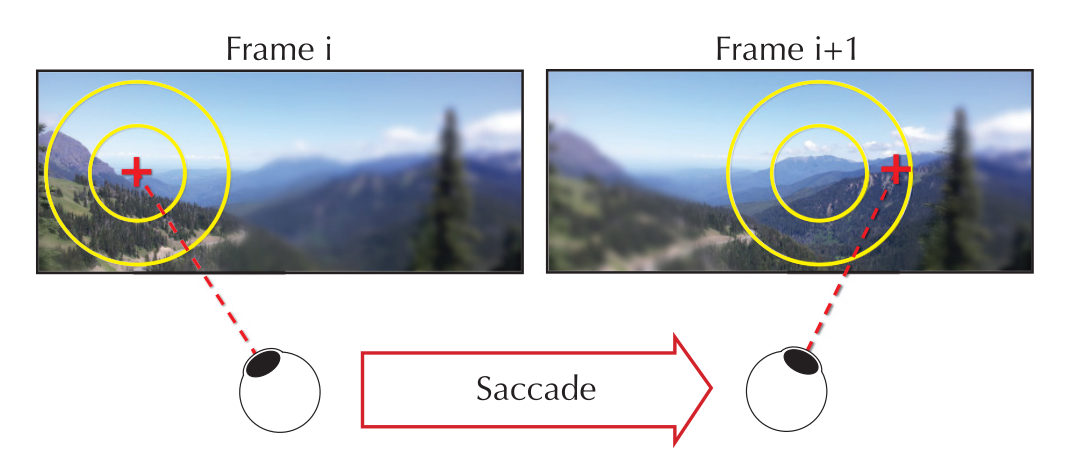
\includegraphics[width=.95\textwidth]{Illustrations/saccade.png}
    \\
    %\tiny{Sam Fraser-Smith \\ \url{http://tr.im/pq7l} }
  \end{center}
  
\end{frame}

%\section[Background]{Virtual Reality Headsets}

\subsection{Virtual Reality Headsets}

\begin{frame}
  \frametitle{Virtual Reality}
  
  	\begin{center}
    		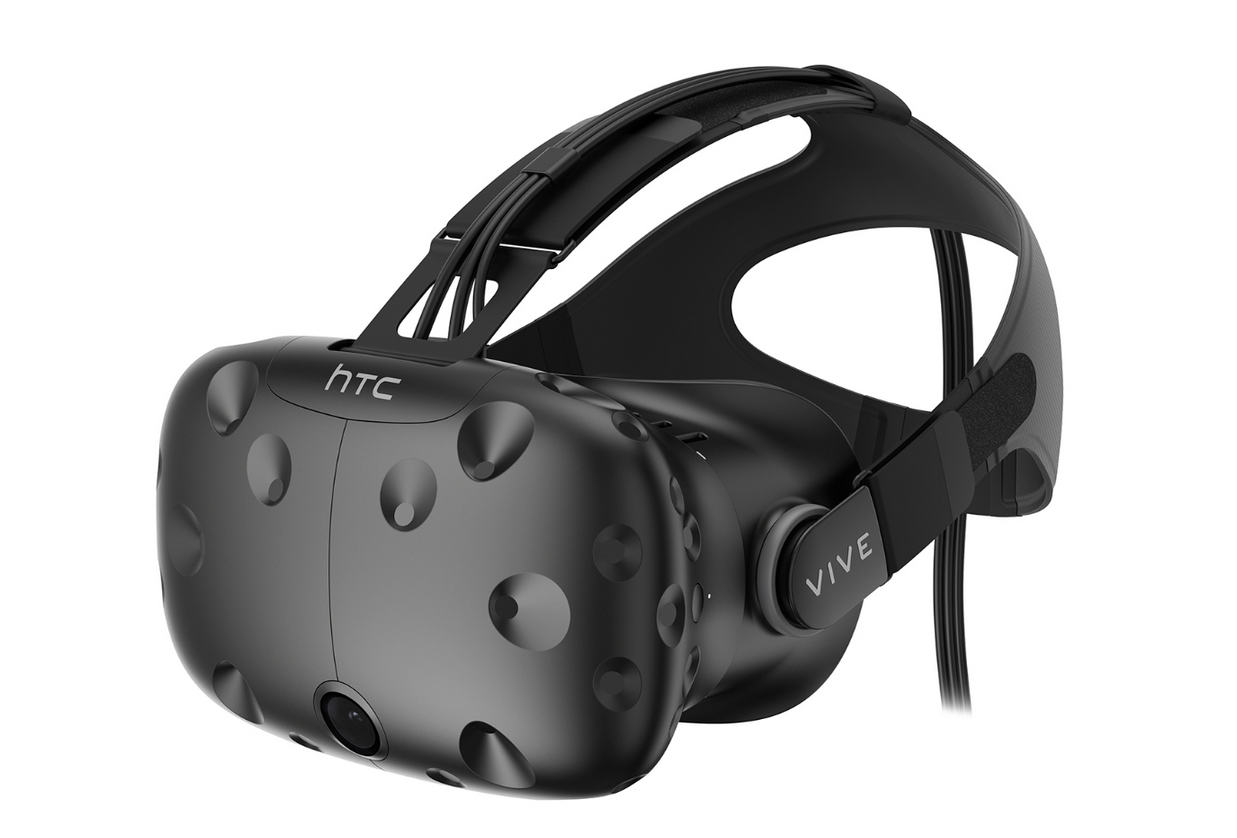
\includegraphics[width=.70\textwidth]{Illustrations/vive.png}
    		\captionof{figure}{HTC Vive}
  	\end{center}
  
\end{frame}

\begin{frame}
  \frametitle{VR Expansion}
	\begin{itemize}
		\item Increased corporate and commercial presence
	\linespace
		\item Options available for a variety of markets
			\begin{itemize}
				\item Enthusiast options like Oculus Rift and the HTC Vive
				\item Casual options like the Samsung Gear VR and Google Carboard
			\end{itemize}
	\linespace 
		\item VR applications demand complex scenes to be generated at high resolutions			
	
	\end{itemize}
\end{frame}


%\section[Background]{Gaze Tracking}

\subsection{Gaze Tracking}

\begin{frame}
  \frametitle{Gaze Trackers}
  
  	\begin{center}
    		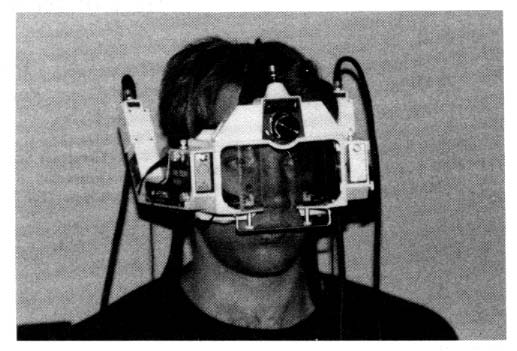
\includegraphics[width=.70\textwidth]{Illustrations/gazeTracker.png}
    		\captionof{figure}{NAC Eye Mark Eye Tracker from the 1980's}
  	\end{center}
  
\end{frame}

\begin{frame}
  \frametitle{Modern Gaze Trackers}
  
  	\begin{center}
    		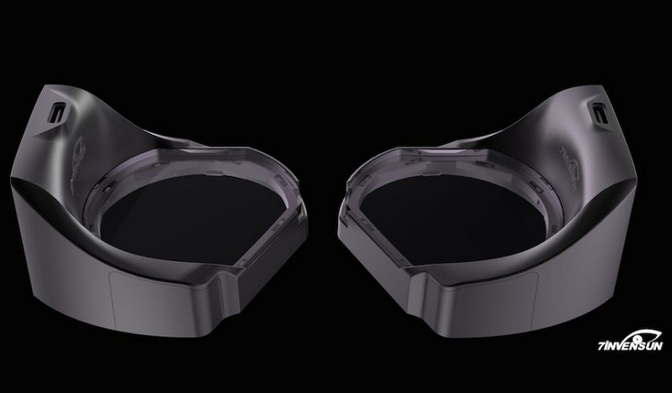
\includegraphics[width=.75\textwidth]{Illustrations/7invensun_aglass2.png}
    		\captionof{figure}{7invensun's aGlass}
  	\end{center}
  
\end{frame}

\begin{frame}
  \frametitle{Hardware Advances}
  
  	\begin{center}
    		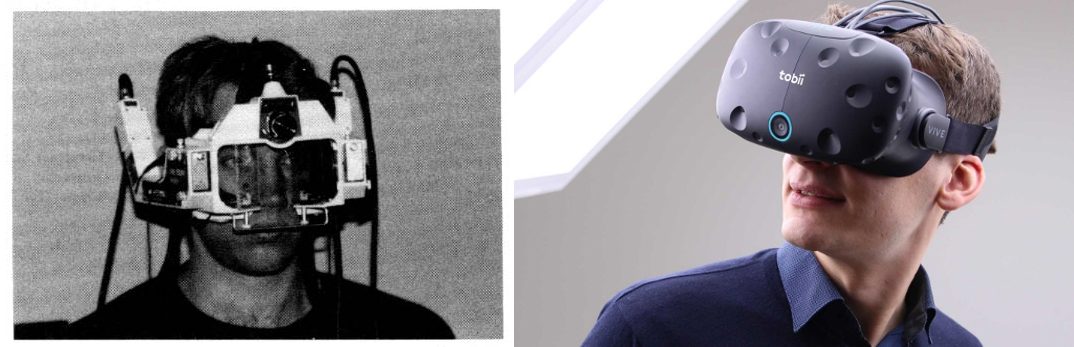
\includegraphics[width=.85\textwidth]{Illustrations/tobii_NAC.png}
    		\captionof{figure}{Comparison of NAC Eye tracker and Tobii VR pro Vive}
  	\end{center}
  
\end{frame}


\section[Foveated Renderer Design]{FR design}

\subsection{Rendering Components}

\begin{frame}
  \frametitle{Problems to address}
	\begin{columns}
	\begin{column}{0.4\textwidth}
	\begin{itemize}
  		\item Aliasing: imperfections generated due the digitization of analogue source material
		\item Spatial or temporal artifacts: aberrations due to the result of distorting processes (like aliasing)
	\end{itemize}
	\end{column}
	\begin{column}{0.6\textwidth}
		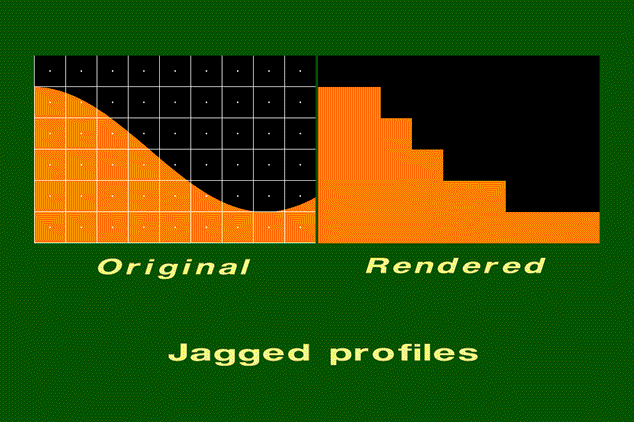
\includegraphics[width=0.95\textwidth]{Illustrations/aliasing.png}
%       \\
%    \only{\tiny{Bluedrakon \\ \url{http://tr.im/pWUi} }}
  	\end{column}
  	\end{columns}
\end{frame}

\begin{frame}
  \frametitle{Aliasing in Foveation}
  
  	\begin{center}
    		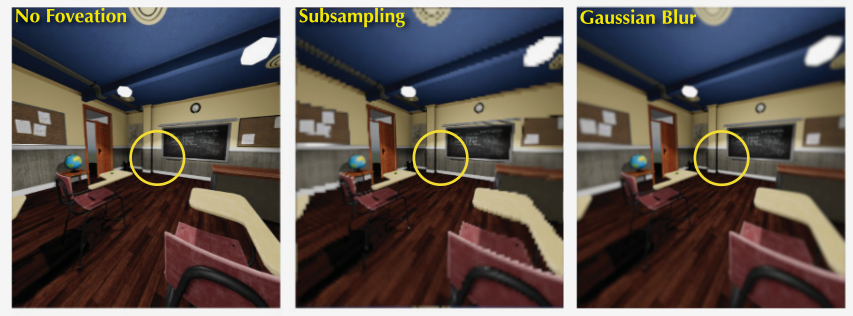
\includegraphics[width=1\textwidth]{Illustrations/foveation.png}
    		\captionof{figure}{Scene render during multiple stages of foveation.}
  	\end{center}
  
\end{frame}


\begin{frame}
  \frametitle{Rendering Tools}
	\begin{itemize}
		\item Anti-Aliasing: methods of reducing aliasing, smoothing the jagged edges
			\begin{itemize}
				\item Multi-Sample Anti-Aliasing (MSAA)
			\end{itemize}
	\end{itemize}
\end{frame}

\begin{frame}
  \frametitle{Rendering Tools Continued}
  
 	 \begin{center}
  		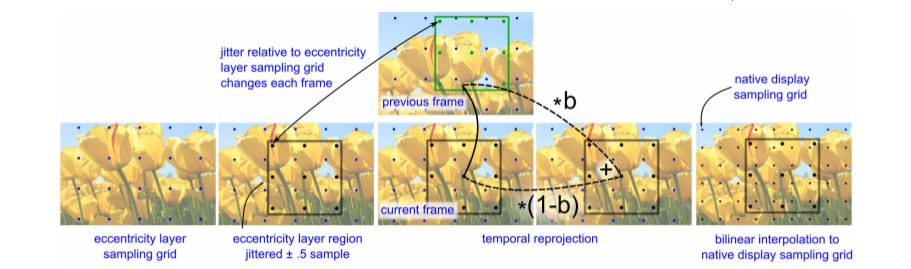
\includegraphics[width=\textwidth]{Illustrations/jitter.png}
  	\end{center}
  	
	\begin{itemize}
		\item Temporal jitter of the spatial sampling grid
		\item Temporal reverse reprojection
	\end{itemize}
\end{frame}

\subsection{Desktop Implementation}
\begin{frame}
  \frametitle{Desktop Implementation}
	\begin{itemize}
		\item Developed by Guenter et al. in 2012
		\linespace
		\item Produced results indistinguishable from non-foveated scenes
		\linespace
		\item Utilized MSAA, temporal reverse reprojection, and sample jittering to combat aliasing
	\end{itemize}
\end{frame}

\begin{frame}
  \frametitle{Desktop Implementation Continued}
	\begin{itemize}
		\item Rendered scenes with three different foveal layers
		\linespace
		\item Reduced the number of pixels shaded by a factor of 10-15
		\linespace
		\item Limited by hardware that is outdated by modern implementation standards
	\end{itemize}
\end{frame}

%\begin{frame}
%  \frametitle{Desktop Implementation}
%	\begin{itemize}
%		\item used retinal eccentricity as a model for visual acuity falloff 
%		\item handled aliasing in the periphery by 
%	\end{itemize}
%\end{frame}


\subsection{Virtual Reality Implementation}

\begin{frame}
  \frametitle{Virtual Reality Implementation}
	\begin{itemize}
		\item Developed by Patney et al.
	\linespace
		\item Directly references the design of Guenter et al.
	\linespace
		\item Applies the technique of foveated rendering to scenes in Virtual Reality
	\end{itemize}
\end{frame}

\begin{frame}
  \frametitle{Virtual Reality Implementation Continued}
	\begin{itemize}
		
		\item Utilized a piecewise linear variation of shading rate
		\linespace
		\item Favored the preservation of contrast 
		\linespace
		\item Created a perceptual visual target in development process	
		%rather than foveal layers (limited some of the temporal aliasing found in Guenters implementation

	\end{itemize}
\end{frame}

\begin{frame}
  \frametitle{Sampling Factors}
  
  	\begin{center}
    		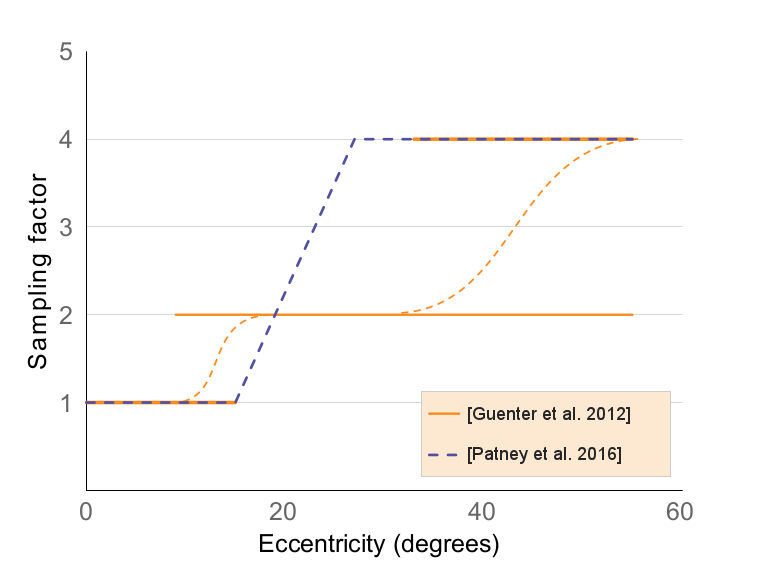
\includegraphics[width=.65\textwidth]{Illustrations/sampling_eccentricity_Patney2.png}
    		\captionof{figure}{Comparison of the rate at which the sampling factor is changed in both implementations.}
  	\end{center}
  
\end{frame}


\section[Results]{User Study Results}



\subsection{User Study Setup}

\begin{frame}
  \frametitle{Patney et al. User Study}
	\begin{itemize}
		\item Patney et al. conducted a user study of both their system and that of Guenter et al.
\linespace		
		\item Both systems were applied to a VR HMD setup to be effectively compared
	\end{itemize}
\end{frame}

\begin{frame}
  \frametitle{Virtual Reality Implementation}
	\begin{itemize}
		\item Four subjects
		\item Two-alternative forced choice test 
		\item 200 trials
		\item Scenes used in trials were varied by transition region size
		\item Successful trials were defined as those with small transition region sizes

	\end{itemize}
\end{frame}

\subsection{User Results}


\begin{frame}
  \frametitle{User Study Transition Thresholds}
  
  	\begin{center}
    		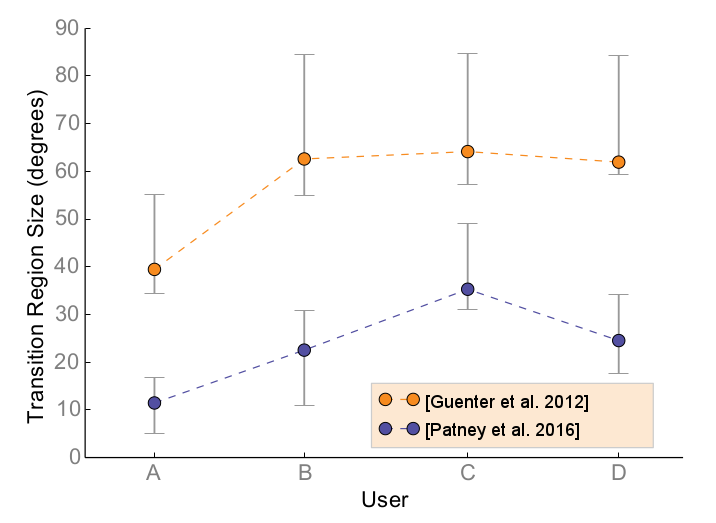
\includegraphics[width=.70\textwidth]{Illustrations/transition_region_Patney.png}
    		\captionof{figure}{Comparison of Transition Region Size used in Patney et al.'s user study}
  	\end{center}
  
\end{frame}

\begin{frame}
  \frametitle{Study Results}
	\begin{itemize}
		\item Users tolerated higher rates of foveation in by Patney et al.'s system
		\item Validates the approach of minimizing temporal artifacts and preserving contrast
		\item Patney et al. were able to shade 70 percent less pixel quads than the non-foveated scene.
		\item Able to use lower quality shading up to 30 degrees closer to the fovea than Guenter et al.
	\end{itemize}
\end{frame}

%%%%%%%%%%%
\iffalse

  
\end{frame}

\begin{frame}
\frametitle{Hardware advancement}

\begin{columns}
\begin{column}{0.5\textwidth}

\begin{itemize}
	\item Early implementations of this technique used hardware such as the NAC Eye Mark eye Tracker (pictured top right).
	\linespace
	\item Current implementations (as of 2017) can use the existing setup of high profile VR HMDs.
	\linespace
	\item This technology is becoming more in demand as the VR userbase expands.
\end{itemize}
\end{column}

\begin{column}{0.02\textwidth}
\end{column}

\begin{column}{0.5\textwidth}

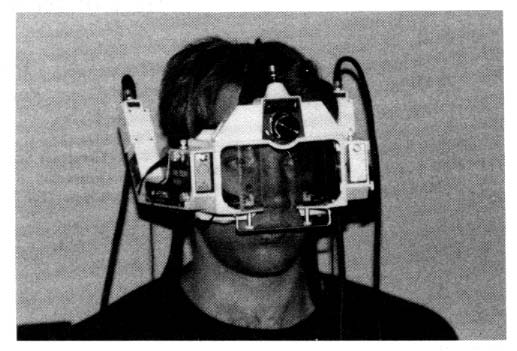
\includegraphics[width=0.715\textwidth]{Illustrations/gazeTracker.png}

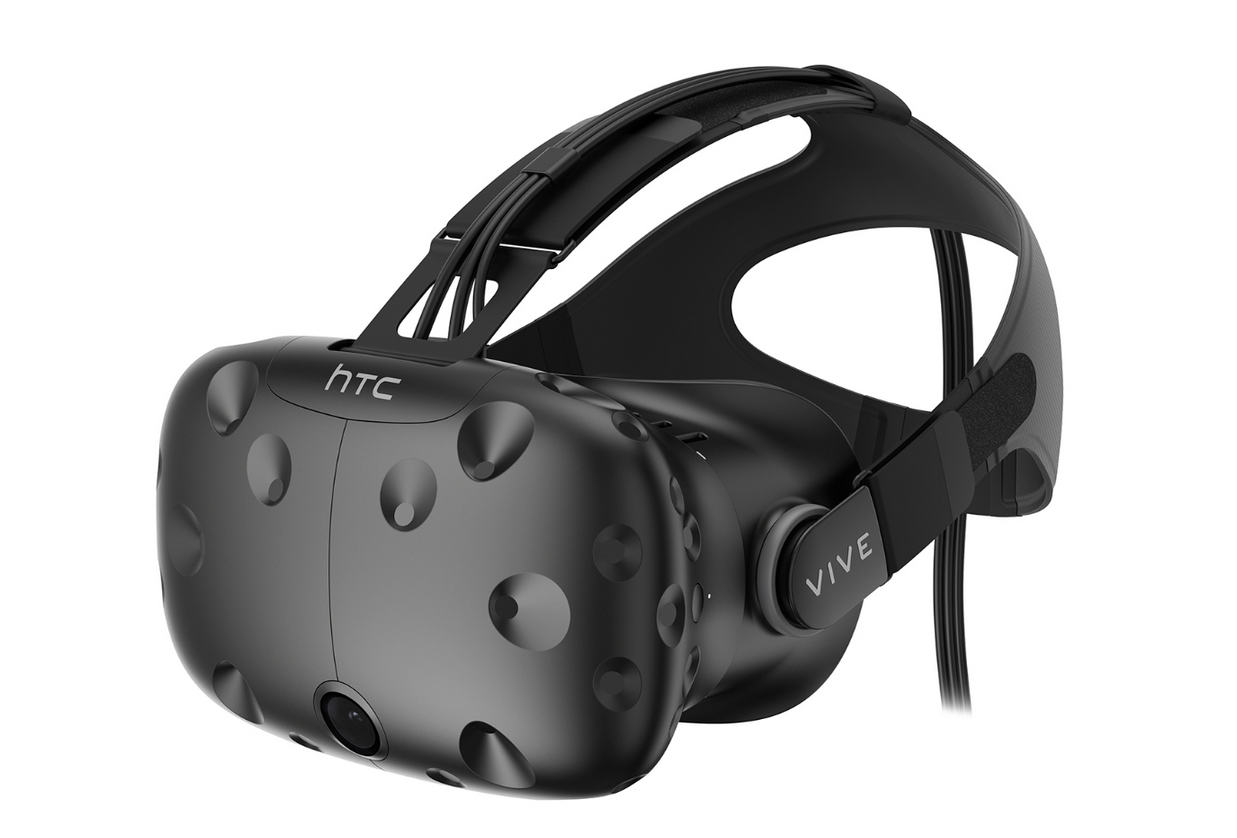
\includegraphics[width=0.715\textwidth]{Illustrations/vive.png}

\end{column}
\end{columns}

\end{frame}

\fi


%%%%%%%%%%%%%%%%%%%

\section[Conclusion]{Questions}

\begin{frame}
	\frametitle{Looking Forward}

	\begin{itemize}
		\item The hardware required for foveated rendering is becoming more common
		\item contrast-preserving temporally-stable foveation implementations have been proven to work
		\item As scene complexity increases, optimization methods suchs as foveated rendering will become more in demand
		\item The systems involved in this process can be applied to other problems
	\end{itemize}
	
\end{frame}



\begin{frame}
	\frametitle{Thanks for listening}

	\begin{center}
	{\huge Questions?}
	\end{center}
\end{frame}


\begin{frame}[t,allowframebreaks]
\frametitle{References}
\bibliography{frvr_talk}
\end{frame}


\end{document}
